\section{Μικρή Aκολουθία}


Η παραγωγή των δύο ακολουθιών βασίζεται σε διαφορετικό αλγόριθμο διάσχισης του συνόλου δεδομένων, ανάλογα με το μέγεθος της ακολουθίας.

Ο αλγόριθμος για την παραγωγή της πρώτης ακολουθίας βασίζεται στη χρήση ενός χρονικού παραθύρου το οποίο μετακυλίεται εντός του συνόλου δεδομένων, αποφασίζοντας άπληστα την αγοραπωλησία μετοχών των διαθέσιμων εταιρειών.
Ο καθορισμός του χρονικού παραθύρου βασίζεται στις δεδομένες σταθερές του προβλήματος, συνεπώς είναι υπολογίσιμος στατικά (εν προκειμένω είναι $40$ ημέρες).

Η βασική λογική είναι ότι λαμβάνει χώρα πάντα μία αγοραπωλησία μετοχών μίας εταιρείας ανά χρονικό παράθυρο.
Η αγορά των μετοχών της εκάστοτε εταιρείας γίνεται κάποια ημέρα του χρονικού παραθύρου στην ελάχιστη καταγραφείσα τιμή μετοχής της εταιρείας, και η αντίστοιχη πώλησή τους λαμβάνει χώρα σε κάποια από τις επόμενες ημέρες στην μέγιστη καταγραφείσα τιμή μετοχής της εταιρείας.
Η επιλογή της εταιρείας μεταξύ όλων όσων είναι διαθέσιμες στο εκάστοτε χρονικό παράθυρο πραγματοποιείται υπολογίζοντας τη μέγιστη διαφορά τιμών μετοχής ανά εταιρεία για το χρονικό παράθυρο, και μετέπειτα σταχυολογώντας τις ευρεθείσες διαφορές (με πολλαπλά κριτήρια, όπως κατά πόσον είναι εφικτή η αγορά τους, κατά πόσον είναι επικερδής η αγοραπωλησία, λαμβάνοντας υπ'όψιν και την επιβεβλημένη προμήθεια, κλπ) ώστε να προκύψει μία άπληστα βέλτιστη ευκαιρία αγοραπωλησίας μεταξύ των εναπομεινασών.

Σημειώνεται ότι, μολονότι δεν επιχειρείται εύρεση βέλτιστης λύσης, λόγω της Άπληστης φύσης του ανωτέρω περιγραφέντος αλγορίθμου ενδέχεται και να μην εντοπιστεί καμία επικερδής αγοραπωλησία σε κάποια εκ των υπό εξέταση χρονικών παραθύρων, εξασφαλίζοντας τοιουτοτρόπως ότι το υπόλοιπο του λογαριασμού ουδέποτε παρουσιάζει ζημιά, παρότι μπορεί ενίοτε να παραμένει σταθερό.

Επιπροσθέτως, προκειμένου να ελαττωθεί ο χρόνος εκτέλεσης της υλοποίησής μας, μειώσαμε περαιτέρω το σύνολο δεδομένων εισόδου εφαρμόζοντας τον παραπάνω αλγόριθμο μόνο σε ένα υποσύνολο $130$ εταιρειών.
Η επιλογή των εταιρειών εισόδου έγινε κατά κύριο λόγο με τυχαίο τρόπο (λόγου χάριν, όλες οι εταιρείες των οποίων η συντετμημένη γραφή αρχίζει από ``x'', ``y'', ``mo'' και ``oi'', χωρίς κάποιον ιδιαίτερο λόγο).
Παρ'όλ'αυτά, κάποιες επιλέχθηκαν λιγότερο τυχαία λόγω της περιέργειας του γράφοντος να συμπεριλάβει γνωστές διεθνούς βεληνεκούς εταιρείες ποικίλων τομέων δραστηριότητας, αλλά κυρίως του κλάδου της Τεχνολογίας (παραδείγματα είναι οι Alphabet, Amazon, Microsoft, IBM, Oracle, Intel, Cisco, αλλά και οι Coca-Cola, J.P. Morgan, BP, Procter \& Gamble, Disney, και άλλες).

Η περιγραφείσα προσέγγιση εξασφάλισε κέρδος $1870282663.4389617$ ($\approx \num{1.87e+9}$) δολλαρίων (σύμφωνα με τον παρεχόμενο online επικυρωτή) κατόπιν $922$ συναλλαγών.

Στο σχήμα \ref{fig:valuation_small} που ακολουθεί, βλέπουμε το διάγραμμα αποτίμησης για το συνολικό χρονικό διάστημα για το οποίο εργαστήκαμε, σύμφωνα με τον ορισμό της αποτίμησης που περιλαμβάνεται στην εκφώνηση της εργασίας.


\begin{figure}[H]
\centering
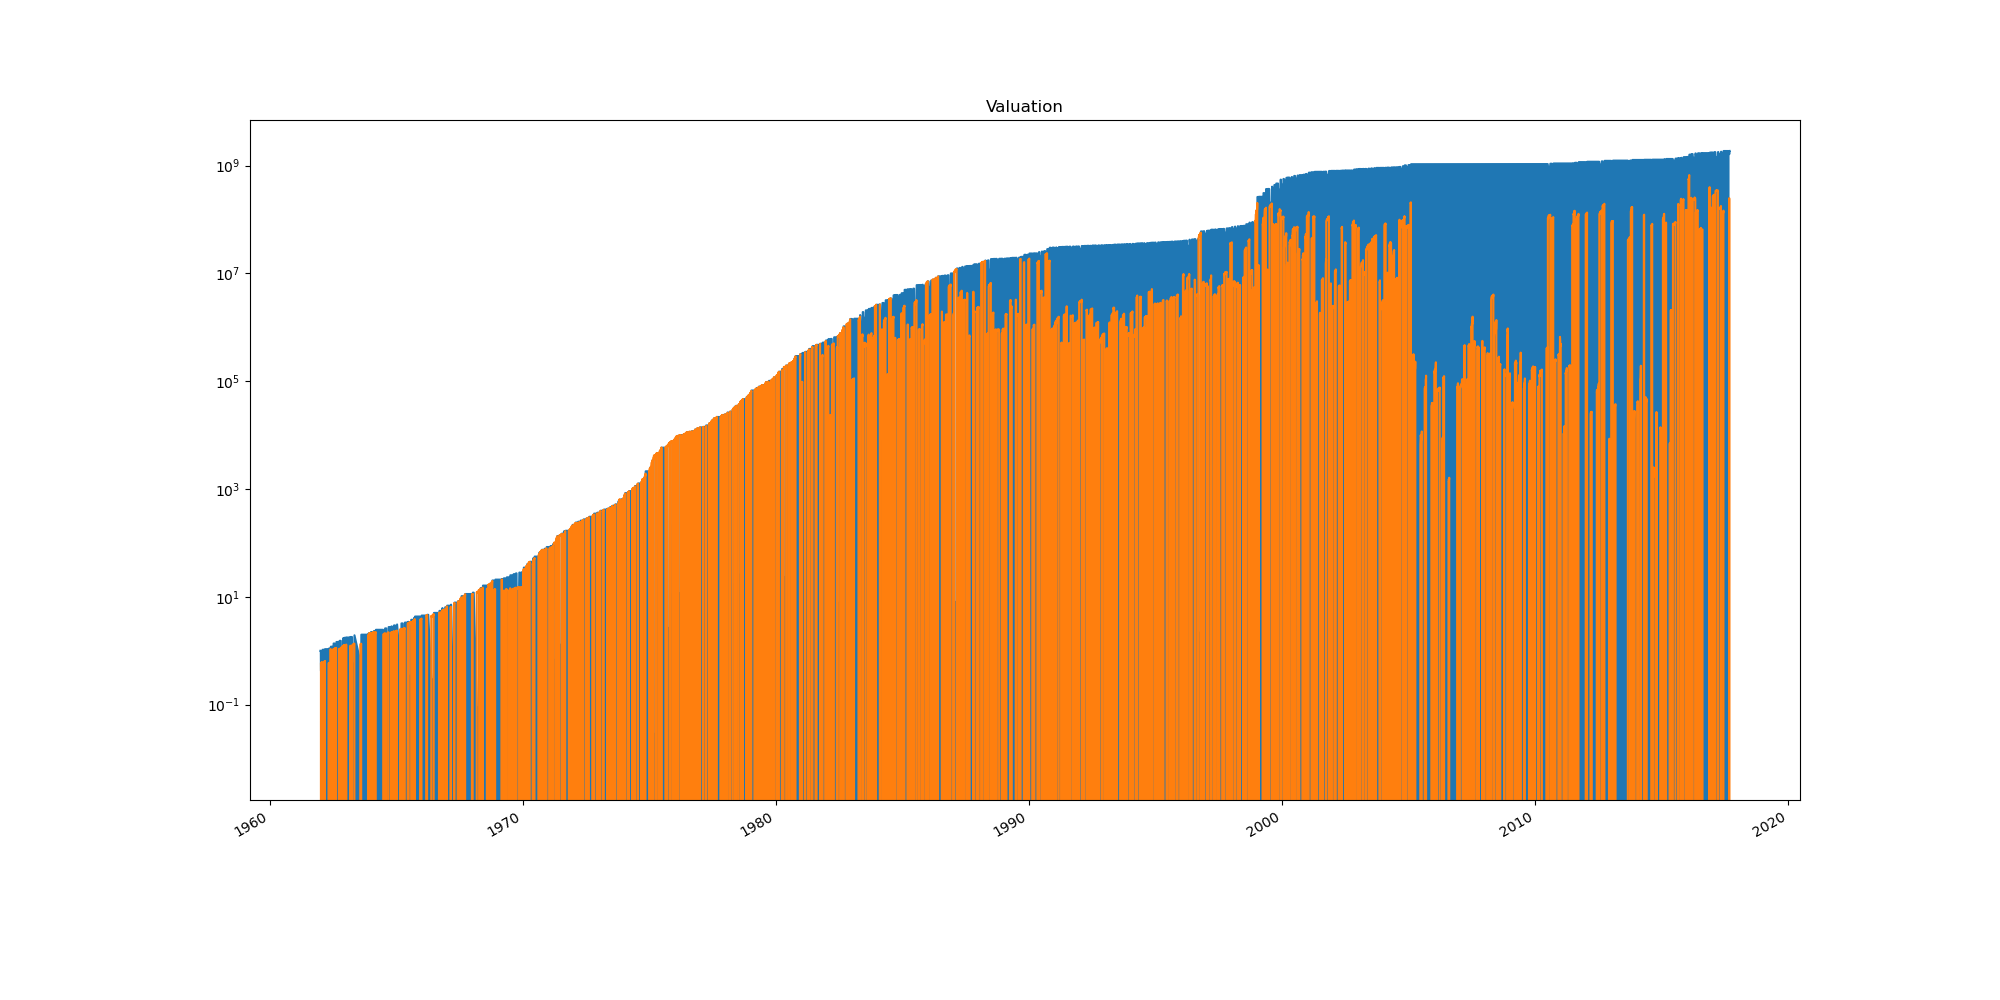
\includegraphics[width=1.1\linewidth]{images/small.png}
\captionof{figure}{Διάγραμμα αποτίμησης κατά τoν υπολογισμό της μικρής ακολουθίας.}
\label{fig:valuation_small}
\end{figure}
